\newcommand{\scripts}{Kapitel 6.}

\chapter{Skripte und Erweiterungen}
\label{chapter:scripts}
\lhead{\scripts \emph{Skripte und Erweiterungen}}

\section{Allgemein}
Neben der Anwendung für den Roboter Pepper und der Webanwendung haben wir weitere Skripte,
hauptsächlich in Python, geschrieben. Diese sind in einem separaten Repository unter
\href{https://github.com/ProjectPepperHSB/Backend-Services}{https://github.com/ProjectPepperHSB/Backend-Services}
zu finden. In diesem Repositry befindet sich, wie in jedem anderen unserer Projekte auch, eine README.md, welche
einen Einstieg in die Installation und Anwendung der einzelnen Skripte ermöglicht.

Es sind mehrere Verzeichnisse angelegt, welche separate Schwerpunkte beinhalten, auf welche wir in den folgenden
Abschnitten genauer eingehen wedern. Auch diese bieten eigene README.md Dateien, welche die Installation, sowie den Zweck aufzeigen.

In jedem dieser kleineren Module befindet sich eine \verb|install.sh|, sowie eine \verb|reguirements.txt| Datei, welche
zusammen ausgeführt werden, um die für das Skript benötigten Packages zu installieren, sofern diese noch nicht vorhanden sind.

Es befindet sich auch ein Verzeichnis mit Namen ``analysis'' in diesem Repository, jedoch gehen wir
darauf im Kapiel \ref{chapter:big-data} genauer ein.

\section{Skripte zur Generierung von Dummy Konversationen}
\label{sec:dummy-data}
Aufgrund der andauernden Einschränkungen der Regierung, ist es uns nicht möglich, Pepper an der Hochschule im vollem Umfang
auszutesten. Somit können wir Pepper und seine Interaktionen nicht an einer großen Menge an Studierenden und Interessierten austesten.
Da wir jedoch den Schwerpunkt Big Data mit in unserem Projekt einfließen lassen wollen und unsere Webanwendung, welche wir im Kapitel \ref{chapter:webapp}
besprochen haben genau für das Sammeln und zur Verfügung stellen von Daten ausgelegt haben, war es für uns ganz klar, dass
wir uns selbst Daten generieren müsssen.

Hierfür wurde ein Skript mit dem Namen \verb|create-dummy-data.py| geschrieben, welches über die Kommandozeile ausgeführt werden kann
und mehrere Parameter übergeben bekommt.

\begin{lstlisting}
    ~$ python3 create-dummy-data.py -n 1000 --prod
\end{lstlisting}

Das Flag \verb|n| gibt die Anzahl der zu generierenden Konversationen an. Das zweite Flag \verb|--prod| ist optioanl und
sorgt dafür, dass die Daten, welche innerhalb des Skriptes generiert werden, an die URL der
laufenden Webanwendung auf dem Hochschulserver gesendet werden. Ohne diesen Flag, werden die Datenreihen an den Localhost geschickt.
Sollte dies nicht einwandfrei laufen, so ist die Webanwendung höchstwahrscheinlich nicht aktiv.

Da die \verb|requests| Library in Python nur synchrone Prozesse unterstützt und dies bei 1000 Anfragen etwas Zeit in Anspruch nimmt,
haben wir dies mit der Library Joblib parallelisiert, sodass 6 Prozesse gleichzeitg die Generierung der Daten, sowie das Übermitteln
an die Webanwendung übernehmen. Aufgurnd der Beschränkungen des Hochschulservers Hopper ist es nicht möglich, noch mehr
gleichzeitige Anfragen zu schicken. Dies ist eine Sicherheitsmaßnahme zur Abwendung von DOS Attacken.


\section{Skripte für die Bereitstellung des Mensaplans}

\newpage
\section{Skripte für die Bereitstellung des 3D-Navigators}

Der Campus unserer Hochschule ist ziemlich weitläufig und unübersichtlich. Dazu kommt, dass mit der Zeit einige Gebäude von der Hochschule als Lernräume angemietet wurden, welche nicht direkt als solche zu erkennen sind. Aufgrund dessen erweist es sich, vor allem für Studenten der ersten Semester, sowie Besucher der Hochschule als äußerst schwierig sich auf dem Campus zu orientieren.
\subsection{Anforderungen}
 Die Benutzer des Roboters sollen die Möglichkeit haben ihn nach einem Raum oder Ort zu fragen und Pepper ihnen daraufhin eine genaue Wegbeschreibung als Antwort geben kann. Dabei ist es von Vorteil, dem Nutzer eine visuelle Beschreibung zu bieten, da die nicht nur einfacher zu verstehen ist, sondern auch mögliche Sprachbarrieren ausschließt. Dafür soll das Tablett von Pepper als visuelle Kommunikation für die Wegbeschreibung dienen. Per Sprache soll Pepper zudem eine geschätzte Dauer des Weges, sowie die Entfernung zu dem gesuchten Ort geben. Außerdem ist es wichtig, dass Pepper auch in der Lage ist barrierefreie Wege für den Benutzer zu beschreiben, da unsere Hochschule weitestgehend auch barrierefrei passierbar ist und körperlich beeinträchtigte Menschen nicht von einem solchen System nicht ausgeschlossen werden sollten.
\subsection{Vorhandene Ressourcen}
Bei der Suche im Web sind die ersten Ergebnisse für eine Orientierungshilfe oder einem Campusplan, die von der Hochschule Bremerhaven unter der offiziellen Internetseite hs-bremerhaven.de bereitgestellten Geländepläne. Diese bestehen aus einem 2-Dimensionalen Campusplan, wie in (Abb. 1) zu sehen, sowie einen 3-dimensionalen Campusplan (Abb 2).

\begin{figure}[H]
    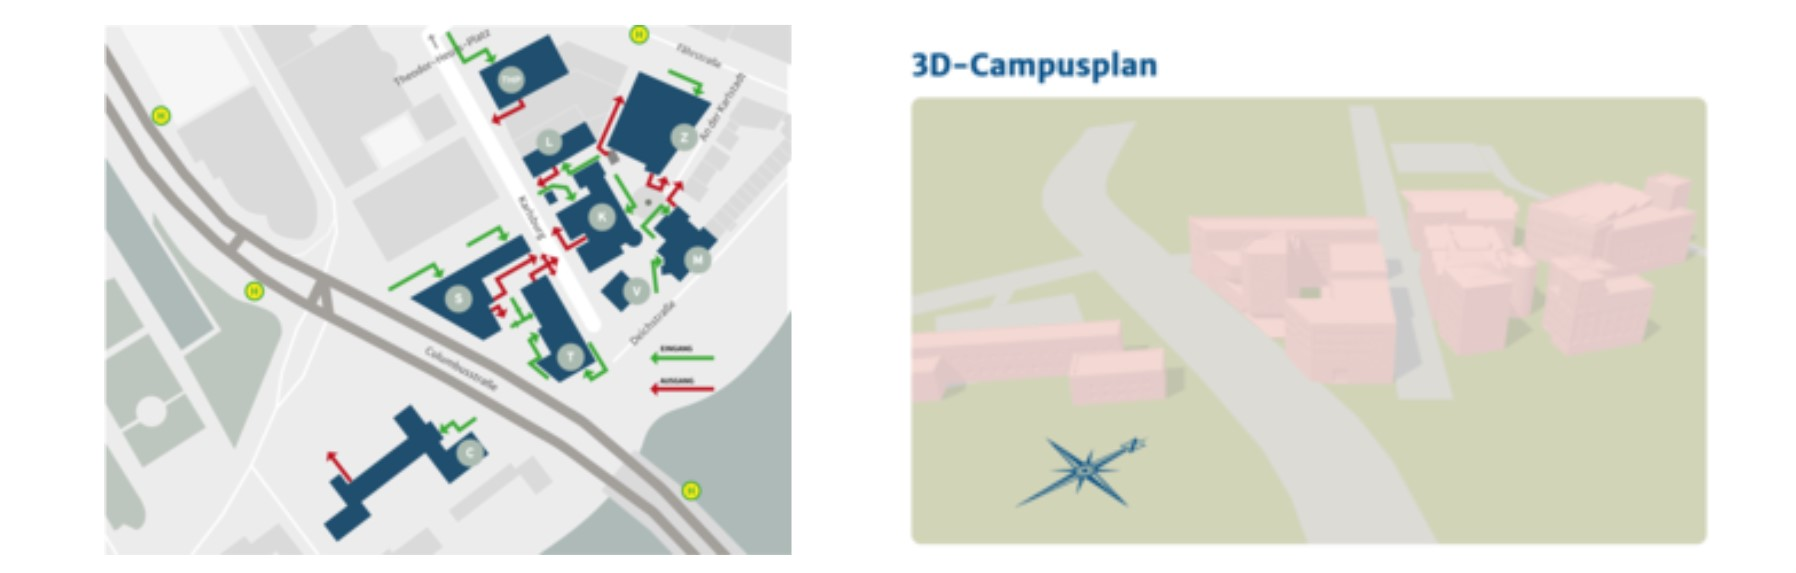
\includegraphics[width=\textwidth]{Figures/3DNavigator/campusplan_bsp.jpg}
    \caption{Beispiel: Zur Verfügung stehende Campuspläne}
    \label{fig:integration}
    \centering
\end{figure}

Zudem wird auch vom AStA Bremerhaven ein Campusplan bereitgestellt.

\begin{figure}[H]
    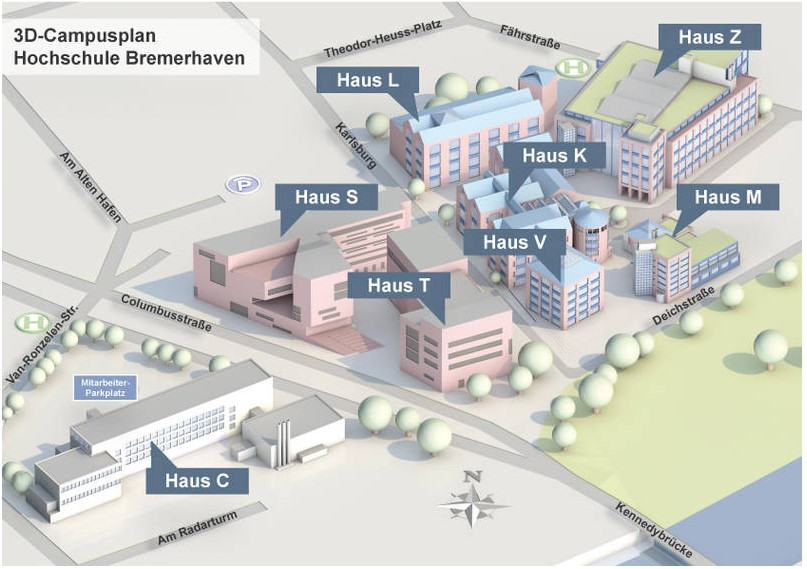
\includegraphics[width=\textwidth]{Figures/3DNavigator/asta_campusplan.jpg}
    \caption{Beispiel: AStA Campusplan}
    \label{fig:integration}
    \centering
\end{figure}

Alle diese Karten haben gemeinsam, dass sie einem zwar einen Überblick über das Campusgelände bieten, wodurch eine nach einem bestimmten Raum suchende Person zwar in der Lage wäre das passende Haus zu finden, allerdings ist es dort angekommen immer noch notwendig den richtigen Raum, mit der entsprechenden Nummer zu finden. Ein weiteres Problem dieser Gebäudepläne ist auch, dass es zwar anhand des Buchstaben vor der zu suchenden Raumnummer möglich ist, das richtige Gebäude zu finden, jedoch nicht, das Haus zu finden, in dem sich beispielsweise die Mensa oder die Bücherei befindet, ohne weitere Recherche zu ermitteln. Da wir vorhaben, dass Pepper den Weg zu einem bestimmten Ort oder Raum genau beschreiben soll, wäre es mit einem solchen Campusplan ein ziemlich großer Aufwand visuelle Markierungen in Form von Linien in die Pläne abbilden zu lassen. Außerdem wäre damit immer noch das Problem der genauen Route innerhalb eines Gebäudes, vor allem für barrierefreie nicht vollständig gelöst. Zudem müssten wir die sprachlich ausgegebenen Informationen zu den Wegrouten selbst erzeugen, was einen sehr großen Aufwand darstellen würde.

Aufgrund dieser genannten Gründe eignet sich also ein solcher Gebäudeplan relativ schlecht für unser Vorhaben, Pepper sinnvoll und effizient für die 3D-Navigation auf dem Campusgelände zu nutzen. Wir haben uns deswegen für eine von 3D-Berlin zur Verfügung gestelltes schlüsselfreies API-System entschieden. Diese API wurde von Prof. Dr.-Ing. Peter Ritzenhoff 2014 im Auftrag der Hochschule Bremerhaven von der 3d-berlin vr solutions GmbH erstellt. Sie besteht aus einem in 3D visualisierten Modell der Hochschule Bremerhaven, in welchem die Räume anhand der Gebäudepläne Maß getreu nach animiert wurden.

\begin{figure}[H]
    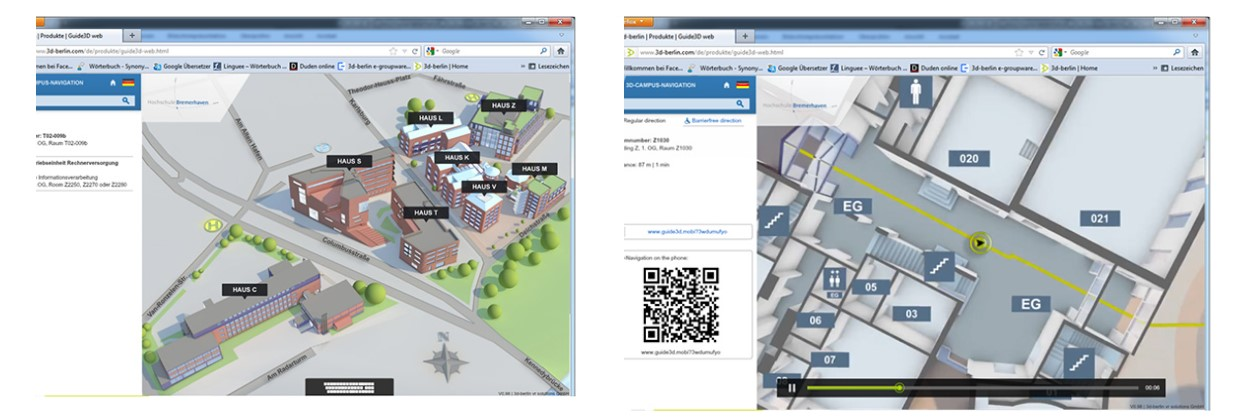
\includegraphics[width=\textwidth]{Figures/3DNavigator/3d-berlin_bsp.jpg}
    \caption{Beispiel: 3d-Berlin 3D-Navigators-API}
    \label{fig:integration}
    \centering
\end{figure}
\vspace{-2.5mm}
Dieses API-System wurde genau für solch einen Anwendungsfall wie wir ihn erstellen wollen entwickelt. Für gewöhnlich werden diese wie von 3d-Berlin entwickelten 3D-Navigation in großen Gebäudekomplexen und Kaufhäusern verwendet, um sie dann auf digitalen Endgeräten wie Smartphones oder Digitalterminals für Besucher zur Orientierung zu Verfügung zustellen (Abb. 5).\vspace{-2.5mm}

\begin{figure}[H]
    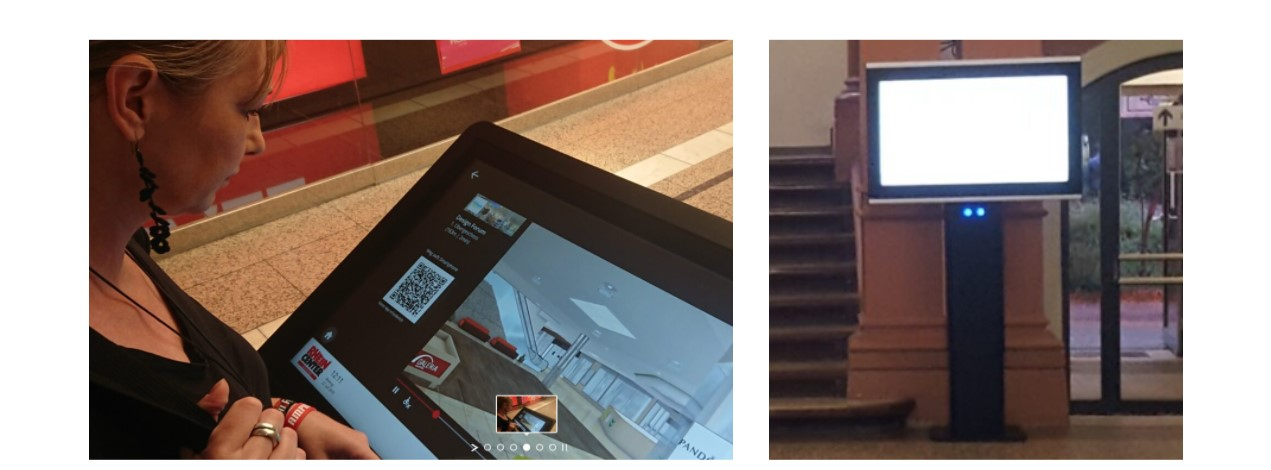
\includegraphics[width=\textwidth]{Figures/3DNavigator/terminal_bsp.jpg}
    \caption{Beispiel: Terminal für Kaufhäuser}
    \label{fig:integration}
    \centering
\end{figure}

Die Implementierung und produktive Verwendung eines solchen 3D-Navigators stellt also eine innovative Anwendung dar. Wir verfügen mit dieser API über die Möglichkeit einen Start,- und Endpunkt als Request an die API zu übergeben und daraufhin per HTTP ein passendes Video mit dem genauen Ablauf der Route zurückgesendet zu bekommen. Ein weiterer Vorteil ist, dass die wir die Distanz in Meter, sowie die geschätzte Dauer für eine Route zwischen zwei Räumen abfragen können, wodurch wir diese Informationen von pepper verbal ausgeben können, während das Tablet ein Video für die Wegbeschreibung abspielt. Anschließend zeigt jedes von der API generierte Video einen QR-code mit einem Link zu dem entsprechenden Video. Dieser QR-Code lässt sich von einem Benutzer mithilfe eines Smartphones einscannen, wodurch sich die Route auch nach Antreten des Weges problemlos nachvollziehen lässt. Außerdem ist die API in der Lage ein Video mit der Wegbeschreibung für einen barrierefreien Weg zu erstellen, womit die Nützlichkeit des 3D-Navigators noch mehr Anwendungsbereiche abdeckt.

\subsection{Entwicklung und Implementierung des 3D-Navigators}

Wir haben uns dazu entschieden, die Daten des 3D-Navigators auf einem eigenen Server bereitzustellen. Dies bietet den Vorteil, dass wir nicht unabhängig von der Verfügbarkeit der 3d-berlin API sind. Zudem sind wir so in der Lage, die Struktur der benötigten Daten selbst zu definieren, um sie möglichst effizient von Pepper abrufen zu lassen. Zunächst haben wir das Vorgehen für die Erstellung des Navigators geplant, wobei wir es für sinnvoll erachten, das Vorgehen in 5 verschiedene Schritte aufzuteilen. Die Abbildung zeigt die chronologische Vorgehensweise bei der Entwicklung, sowie die primär verwendete Programmiersprache, so wie weitere benötigte Technologien, um das Ziel des jeweiligen Schrittes zu erreichen.

\begin{figure}[H]
    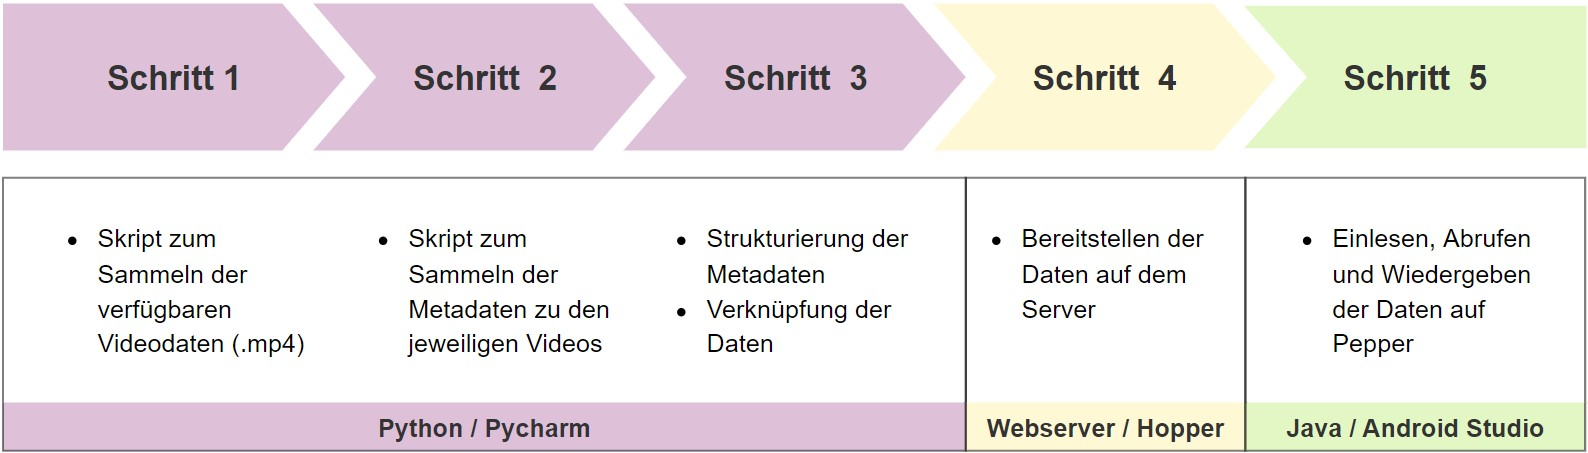
\includegraphics[width=\textwidth]{Figures/3DNavigator/Implementierungdes3DNavigators.jpg}
    \caption{Vorgehen: Entwicklung des 3D-Navigators}
    \label{fig:integration}
    \centering
\end{figure}

\subsubsection{Planung der Videodaten-Struktur}

Die Strukturierung der Videos soll so erfolgen, dass es bei der fertigen Implementierung für die Kommunikation zwischen Pepper und dem Server möglichst unproblematisch, sowie effizient ist, das passende Video zu der benötigten Anfrage abzurufen. Außerdem ist es aufgrund der speziellen Sonderzeichen innerhalb einiger Raumnamen nicht möglich, die Namen der Räume direkt innerhalb der Deklaration der Videodateien zu verwenden. Die Struktur der Dateinamen besteht deswegen aus drei notwendigen Informationen, diese sind dabei der Übersicht halber mit einem „-“ Zeichen voneinander getrennt und bilden immer einen nur einmalig vorkommenden Namen zur Wiedererkennung des jeweiligen Videos. In der ersten Sektion befindet sich die ID für den Startpunkt der Route und in der zweiten die des zu erreichenden Endpunktes. Die Definition dieser IDs sind dieselben ID-Namen, wie sie die API von 3D-Berlin verwendet hat. Das hat den Vorteil, dass wir im Nachhinein besser nachvollziehen können, aus welchen Request das entsprechende Video ursprünglich stammt. Zudem wäre es zeitlich redundant eine neue ID Nummerierung hierzu anzulegen. Der dritte Abschnitt des Videonamen beschreibt, ob es sich um ein Video mit einem Barrierefreien Weg oder um einen gewöhnlichen Weg handelt. Dabei steht die Bezeichnung „M0000“ für den gewöhnlichen Weg und „M0001“ für einen Weg unter Berücksichtigung der Barrierefreiheit. Somit gibt es für jedes Video also zwei verschiedene Varianten. Die untere Abbildung soll eine Abstrahierung dieser Datenstruktur verdeutlichen.\vspace{-2.5mm}

\begin{figure}[H]
    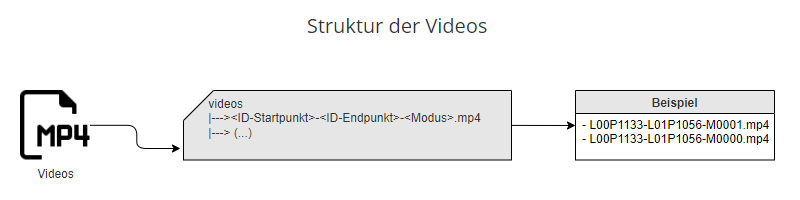
\includegraphics[width=\textwidth]{Figures/3DNavigator/Videostruktur_Raumfinder.png}
    \caption{Datenstruktur: Wegrouten Videos}
    \label{fig:integration}
    \centering
\end{figure}\vspace{-2.5mm}

Bei dem Format der Videos haben wir uns für MP4-Format entschieden. Diese Videodateien verfügen über eine gute Browserkompatibilität und haben trotz einer verhältnismäßig geringen Speichergröße trotzdem eine möglichst hohe Bildqualität. [1] Da wir bei jeder Anfrage an eine Wegbeschreibung das entsprechende Video per http auf von dem Server an den Roboter senden, eignet sich dieses Format also gut, da wir so eine entsprechend geringe Verzögerung beim Übertragen und Anzeigen der Videodatei erreichen. Wir haben uns deswegen für eine Bildbreite von 306px und eine Bildhöhe von 544px entschieden, wodurch wir eine durchschnittliche Größe von 1.5 MB pro MP4-Datei kommen. Insgesamt soll Pepper in der Lage sein ca. 500 verschiedene Wegbeschreibung zu abzubilden, wodurch sich ein Datensatz von ca. 1.000 MP4-Videos mit insgesamt 845 MB Kapazität ergibt.

\subsubsection{Sammeln der Videodaten}

Zunächst haben wir uns einen Überblick darüber verschafft, welche Daten wir mithilfe der 3d-Berlin API erhalten können. Als geeignetes Werkzeug für das automatisierte Arbeiten mit Requests haben wir uns für die Programmiersprache Python entschieden. Python bietet uns die Möglichkeit schnell und zielorientiert ein brauchbares Skript zu schreiben, um die benötigten Daten nicht nur auszulesen, sondern auch zu formatieren und sie später direkt in unsere gewünschte Datenstruktur einzubinden. Das Pythonskript “createvideodata.py” ist Teil unseres Backend-Service und dient dazu, die erforderlichen Requests für den Download der Videos zu konstruieren. Anschließend werden diese ausgeführt und mit dem richtigen Dateinamen zu versehen. Ein paar relevante Ausschnitte des Skripts möchten wir im Folgenden erläutern.
Um genau zu wissen, welche Wegrouten wir erzeugen können, rufen wir zunächst eine Liste der Video-IDs ab. Wir bekommen diese in Form einer JSON-Datei als Response zurück und initialisieren die Variable “videos” mit ihr.

\begin{figure}[H]
    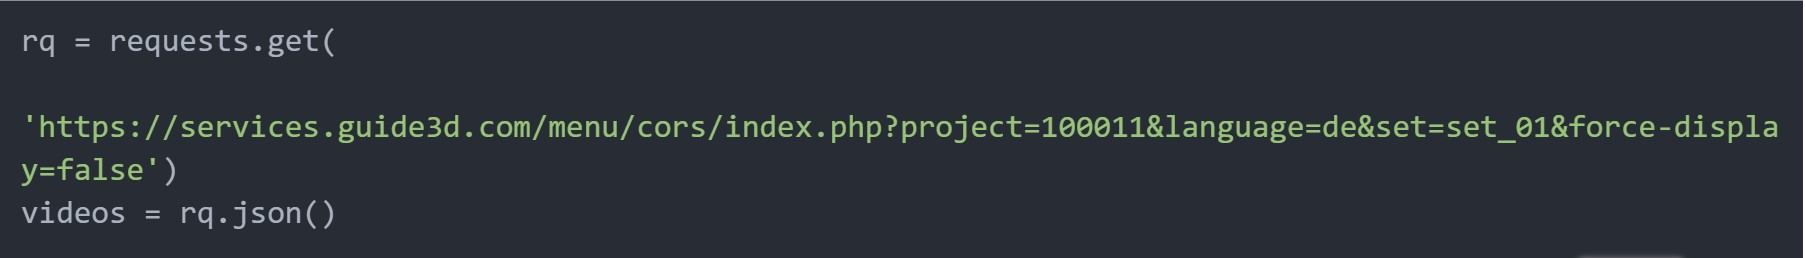
\includegraphics[width=\textwidth]{Figures/3DNavigator/code01.jpg}
    \centering
\end{figure}\vspace{-2.5mm}

Wir definieren außerdem eine variable “directory”, in welcher wir den Defaultwert für das Verzeichnis angeben, in das die Videos später gespeichert werden sollen. Die projekt-id “project” initialisieren wir, um später mögliche Änderungen für weitere Projekte vornehmen zu können. Die hier gewählte ID “100011” ist die des Projektes der Hochschule Bremerhaven. Zusätzlich initialisieren wir die Domain zu der API von 3d-Berlin in der variable “url”.

\begin{figure}[H]
    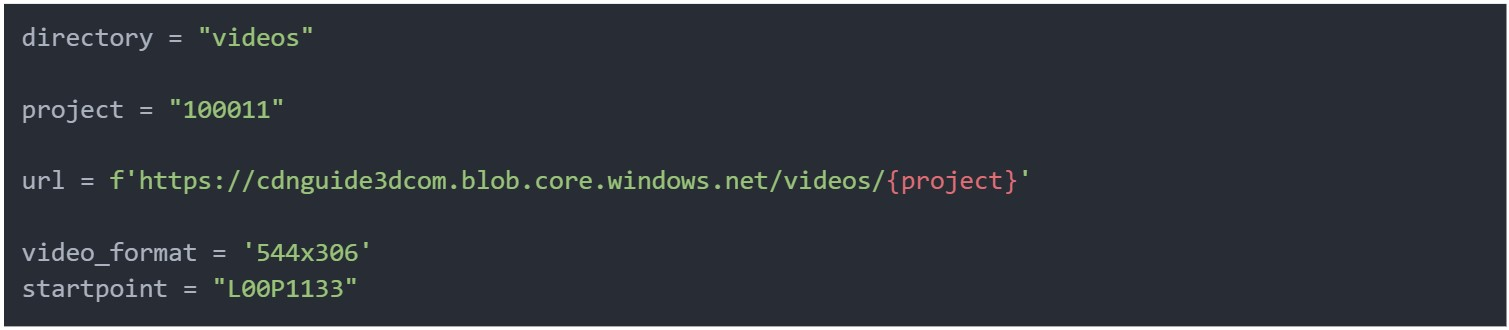
\includegraphics[width=\textwidth]{Figures/3DNavigator/code02.jpg}
    \centering
\end{figure}\vspace{-2.5mm}

Den wohl relevantesten Teil des Skripts stellt die folgende for-Schleife dar. Hier iterieren wir über die in der zuvor eingelesenen JSON-Datei angegebene Liste der Räume, zu welchen es Informationen in Form einer Wegbeschreibung gibt. Wir leiten daraus ab, dass wir zu jedem dieser Einträge auch ein Video von der API anfordern können. Dazu lesen wir bei jedem Eintrag eines Videos die dazugehörige ID des Endpunktes der Route, sowie den mit dieser ID verknüpften Namen des Raumes ein und speichern sie jeweils in einer Variable zwischen. Danach übergeben wir die zu der Wegroute entsprechenden Informationen an unsere zuvor definierte Funktion zum Erstellen des Requests. Wir rufen dabei diese Funktion jeweils einmal für den normalen weg und für den Barrierefreien weg auf.

\begin{figure}[H]
    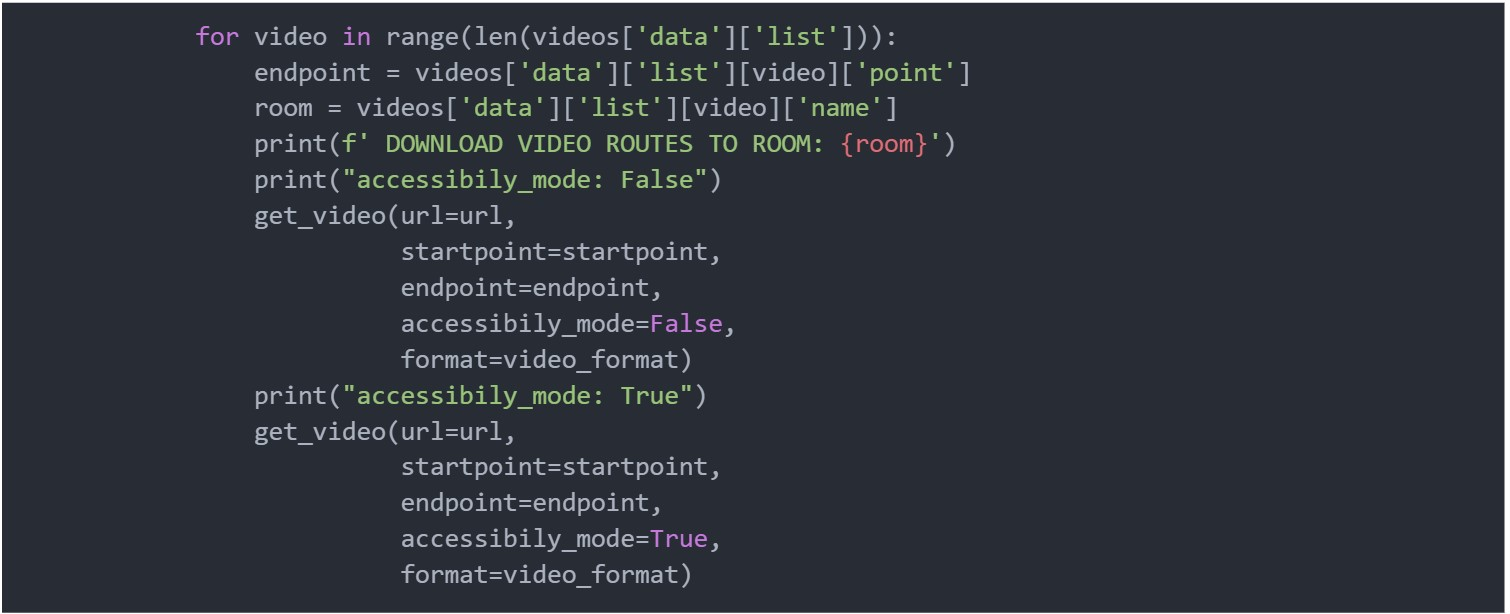
\includegraphics[width=\textwidth]{Figures/3DNavigator/code03.jpg}
    \centering
\end{figure}\vspace{-2.5mm}

Ist ein Request erfolgreich ausgeführt wurden, so speichern wir die erhaltene MP4-Datei zwischen und schreiben sie in das vorab gewählte Verzeichnis für die Videos.

\begin{figure}[H]
    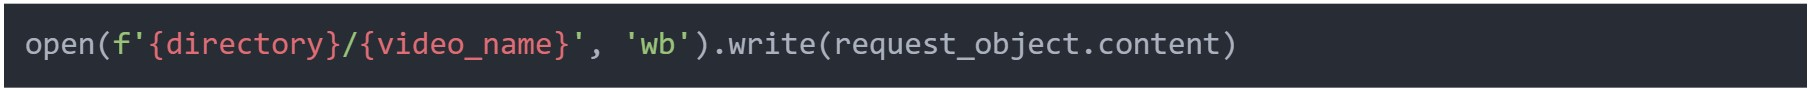
\includegraphics[width=\textwidth]{Figures/3DNavigator/code04.jpg}
    \centering
\end{figure}\vspace{-4.5mm}

Als letztes haben wir das Skript mit Hilfe des “PySimpleGUI”  Frameworks noch um eine Grafische Oberfläche erweitert. Mit diese sind wir in der Lage nachhaltig das Verzeichnis zum speichern der Videos über den windows-explorer auszuwählen. Zudem haben wir einen Ladebalken implementiert, welcher den Fortschritt des Downloads anzeigt. Abbildung 10 zeigt die von uns erstellte grafische Anwendung und den Output des Skripts:

\begin{figure}[H]
    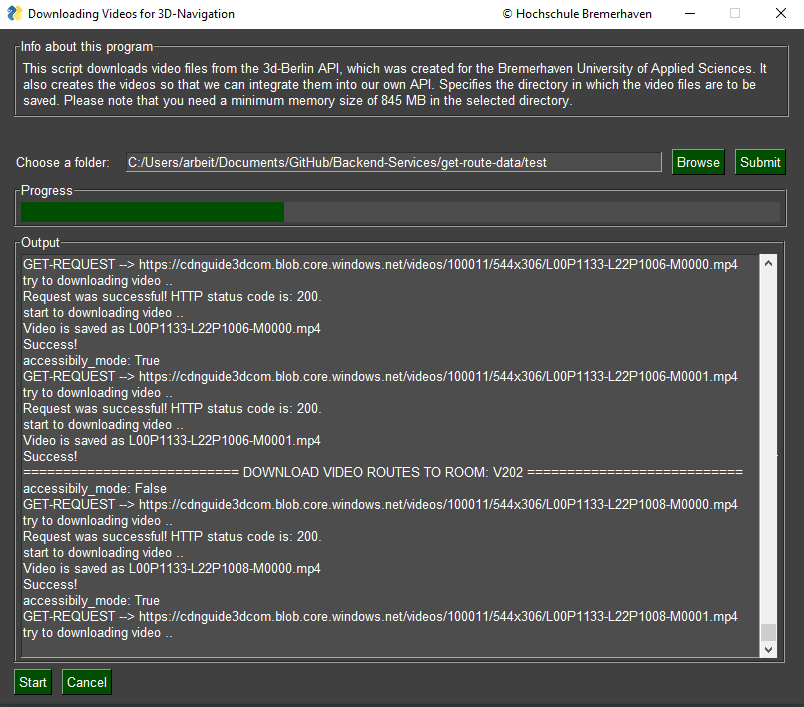
\includegraphics[width=\textwidth]{Figures/3DNavigator/create_videodata_pic.png}
    \caption{Screenshot: Grafische Oberfläche des Download-Skripts}
    \label{fig:integration}
    \centering
\end{figure}\vspace{-2.5mm}

Ist das Skript durchgelaufen haben wir die Videos erfolgreich in die geplante Struktur und mit der korrekten Deklaration der Dateinamen in ein Verzeichnis gespeichert. 

\begin{figure}[H]
    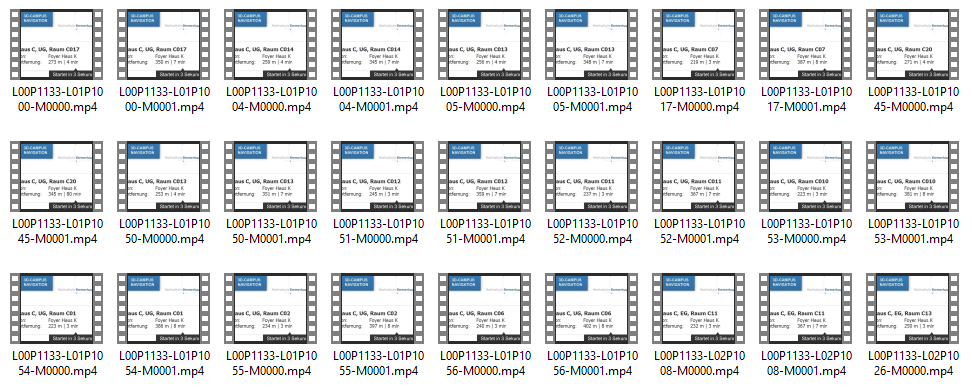
\includegraphics[width=\textwidth]{Figures/3DNavigator/videos.png}
    \caption{Screenshot: Ausschnitt der durch das Skript erstellten Videos}
    \label{fig:integration}
    \centering
\end{figure}\vspace{-2.5mm}

\subsubsection{Planung der Datenstruktur für die Routeninformationen}

Die Strukturierung der Metainformationen soll so gestaltet werden, dass es für Pepper und den Server möglichst einfach ist, das passende Video zu der erfolgten Anfrage abzurufen. Die Metainformationen über die Wegbeschreibungen zu einem Raum setzen sich aus folgenden Attributen zusammen:\vspace{5mm}

\begin{tabular}{| l | p{9.45cm} | c| } \hline 
\multicolumn{3}{|c|}{\textbf{Attribute einer Wegroute}}\\ \hline\hline
Beschreibung & Kommentar & Datentyp \\
\hline
Art des Weges & \small Es gibt zu jeder Wegbeschreibung zwei verschiedene Arten, das Ziel 
zu erreichen. Dabei bilden wir jeweils einen barrierefreien und einen gewöhnlichen 
bzw. schnell zu erreichenden Weg an. Obwohl es nur zwei verschiedene Zustände für die Art eines Videos gibt, haben uns hierbei bewusst für einen String und nicht für einen booleschen Wert entschieden. Der Grund dafür ist, dass sich bei der Erstellung des Skriptes () gezeigt hat, dass wir so keine Datentypen bei der Strukturierung eines Requests umwandeln müssen. Außerdem haben wir so die Möglichkeit über genügend Agilität zu verfügen, sollten wir dieses Skript zukünftig für ein Projekt werden wollen, welches mehr als zwei Modi verwendet. & String\\[0.5ex]
\hline
Videopfad &  \small Dieser Parameter stellt die direkte Verknüpfung zu der entsprechenden Daten mit der dazugehörigen Rauminformation dar. So können wir möglichst präzise das passende Video mit der richtigen Wegbeschreibung ermitteln.
& String\\
\hline
Ort &   \small Der Ort ist eine kurze Beschreibung, in welchem Haus und welcher Etage sich der Raum befindet. Eine solche Ortsbeschreibung wäre zum Beispiel “Haus C Erdgeschoss”. Mit dieser Umschreibung kann Pepper dem Benutzer noch eine zusätzliche Information für eine verbale Interaktion bieten. & String\\
\hline
Distanz & \small Bei der Distanz geben wir die Entfernung, ausgehend vom Startpunkt der Wegbeschreibung bis zum Ziel an. Wir verwenden dabei Meter als Einheit und runden diese für eine bessere Verständlichkeit auf ganze Meter auf. & Integer\\
\hline
Dauer & \small Die Dauer geben wir in Minuten an. Sie beschreibt die benötigte Zeit vom Startpunkt bis zum Ziel, ausgehend von der durchschnittlichen Schrittgeschwindigkeit. & Integer\\
\hline
\end{tabular} \vspace{5mm}

Als Nächstes haben wir damit angefangen, die zur Verfügung stehenden Eigenschaften der Wegrouten sinnvoll miteinander zu verknüpfen und in Relation untereinander zu betrachten. Dabei sei vorausgesetzt, dass die Informationen immer zu genau einem Video gehören und dabei möglichst pragmatisch zu finden sein sollen. Außerdem gibt es zu jedem Raum genau zwei verschiedene Wegbeschreibungen, da wir zwischen dem Normalen und dem Barrierefreien Weg unterscheiden. Dies hat zur Folge, dass zu jeder Wegroute zwei verschiedene Eigenschaften zur Verfügung stellen muss, welche sich jedoch die gleiche Art und Struktur der Datentypen teilen. Diese Beziehungen der Daten zueinander haben wir der Übersicht halber in einem Entity-Relationship-Modell  charakterisiert.

\begin{figure}[H]
    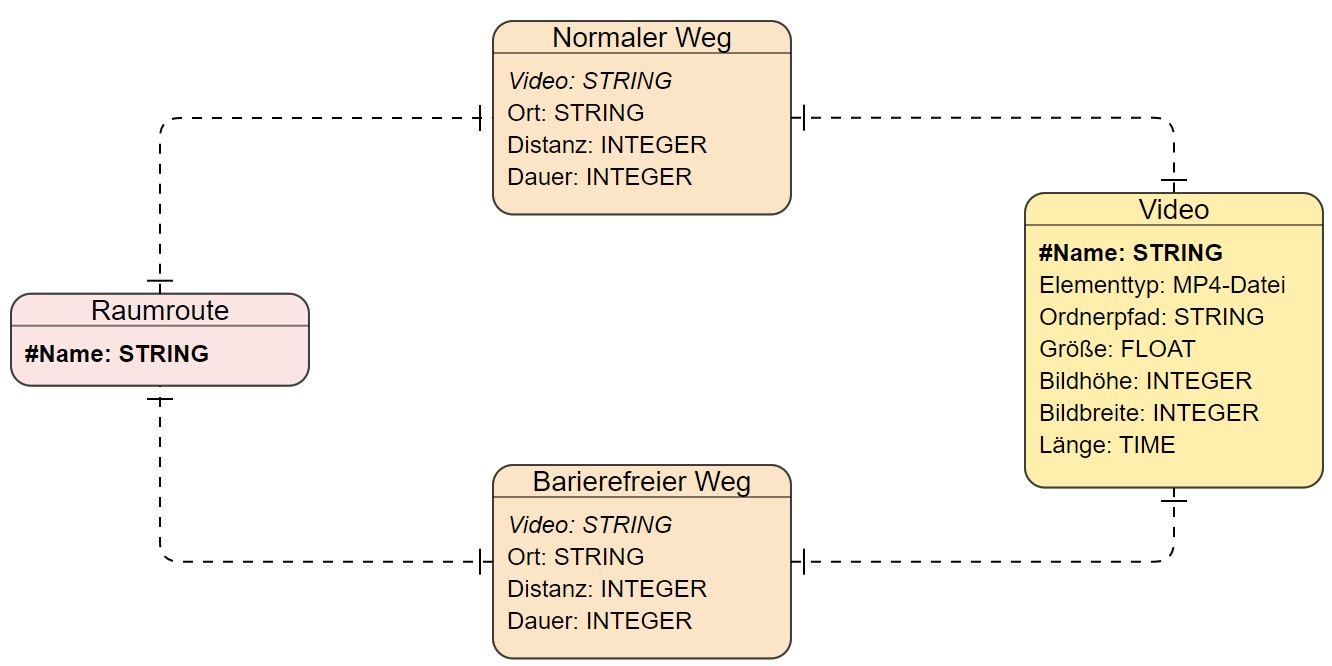
\includegraphics[width=\textwidth]{Figures/3DNavigator/EntityrelationshipdiagrammRaumfinder.jpg}
    \caption{Diagramm: ER-Modell der Wegrouten Informationen}
    \label{fig:integration}
    \centering
\end{figure}

Mithilfe dieses Datenmodells sind wir dazu übergegangen, ein passendes Datenformat für unseren Anwendungsfall zu wählen. Wir haben uns dabei für die JavaScript Object Notation entschieden, da sie uns den Vorteil bietet möglichst einfach und lesbar unsere Datenstruktur abzubilden. Außerdem verfügen wir so über ein Datenformat, welches eine hohe Programmiersprachen-Unabhängigkeit bietet. Dies erweist sich für unsere Architektur als äußerst vorteilhaft, da wir zwischen unseren Anwendungen und Entwicklungsabläufen verschiedene Programmiersprachen verwenden. Die endgültig geplante Datenstruktur der JSON-Datei haben wir unten in der Abbildung unten abstrahiert dargestellt.

\begin{figure}[H]
    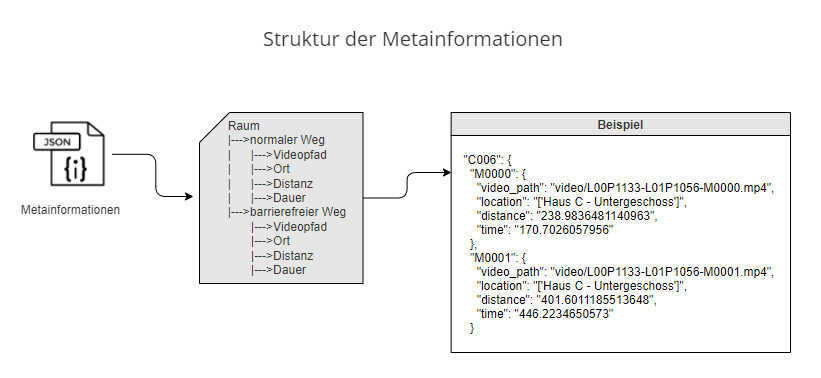
\includegraphics[width=\textwidth]{Figures/3DNavigator/Metadatenstruktur_Raumfinder.png}
    \caption{Datenstruktur: Abstrahierung der Wegrouten Informationen}
    \label{fig:integration}
    \centering
\end{figure}

\subsubsection{Sammeln der Wegroutendaten}

In der Dokumentation von 3d-Berlin wird ausschließlich beschrieben, wie die entsprechenden Request für die zu generierenden Videos zu definieren sind. Aus diesem Grund sind wir so vorgegangen, dass wir mithilfe des Netzwerkanalysetools unseres Browsers die Response der gesendeten Requests, während der Nutzung des 3D-Navigators beobachtet haben. Dabei konnten wir genau ermitteln, welche Requests notwendig sind, um weitere Daten über die Videos zu erhalten und wie diese in ihrer Struktur aufgebaut werden müssen.

\begin{figure}[H]
    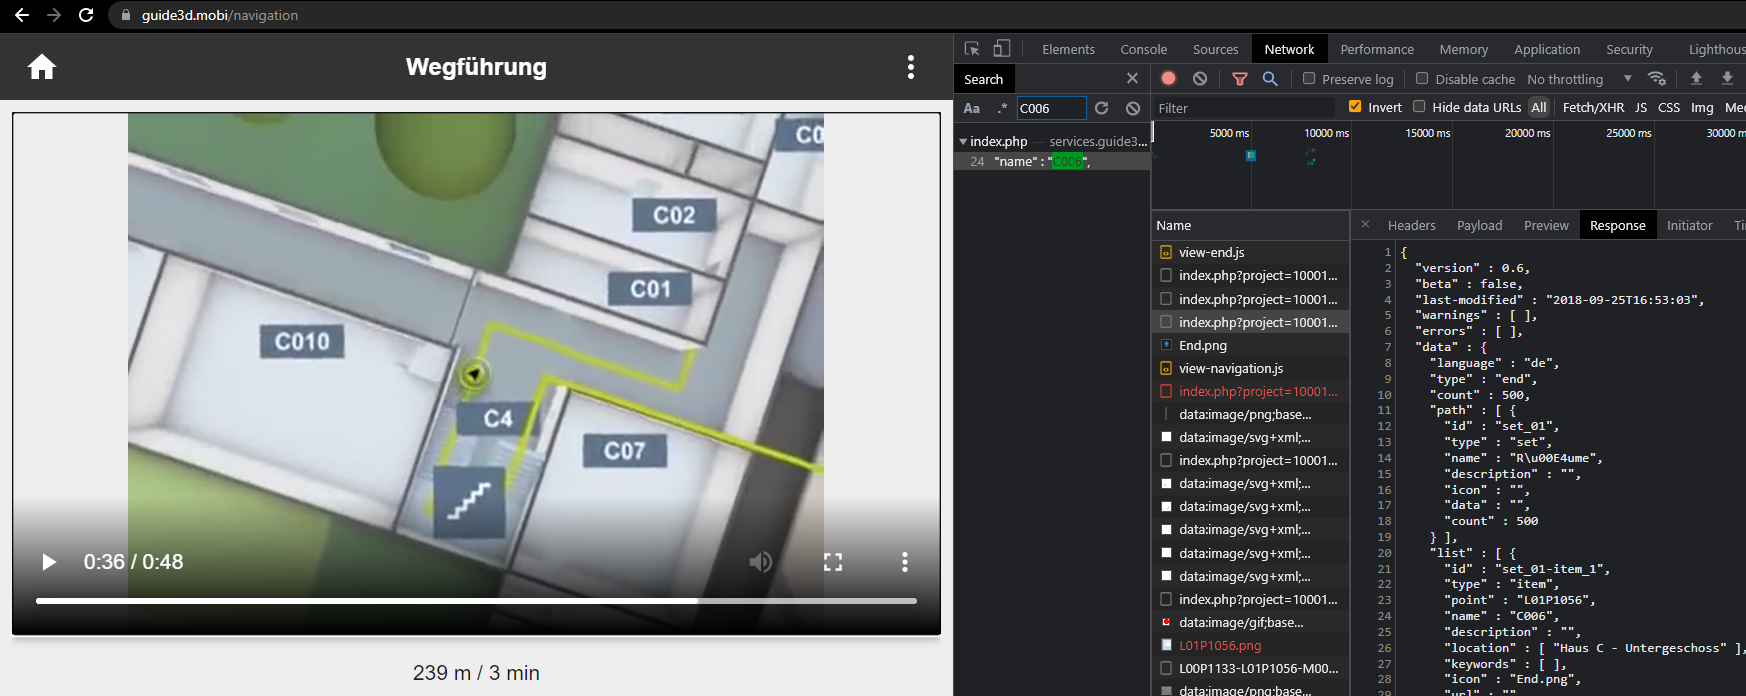
\includegraphics[width=\textwidth]{Figures/3DNavigator/analysetool.png}
    \caption{Screenshot: Google Chrome Netzwerk Analyse Tool}
    \label{fig:integration}
    \centering
\end{figure}

Auch hier haben wir uns für die Programmiersprache Python als passendes Werkzeug entschieden. Dafür haben wir innerhalb unseres Backend-Service ein weiteres Skript namens “createmetadata.py” angelegt. Das Skript beschafft sich die Informationen, welche wir unter der API 3d-Berlin finden konnten und wandelt diese in für uns brauchbare Daten um. Außerdem werden diese anschließend in der Datei “routedata.json” in Java Object Notation gespeichert. Im Folgenden gehen wir auf ein paar relevante Abschnitte des Skripts genauer ein und erläutern diese.

Zu Beginn werden zwei verschiedene Requests definiert. Der Erste erzeugt das Request-Objekt für den normalen Weg und der Zweite generiert das gleiche Request-Objekt als barrierefreie Route.

\begin{figure}[H]
    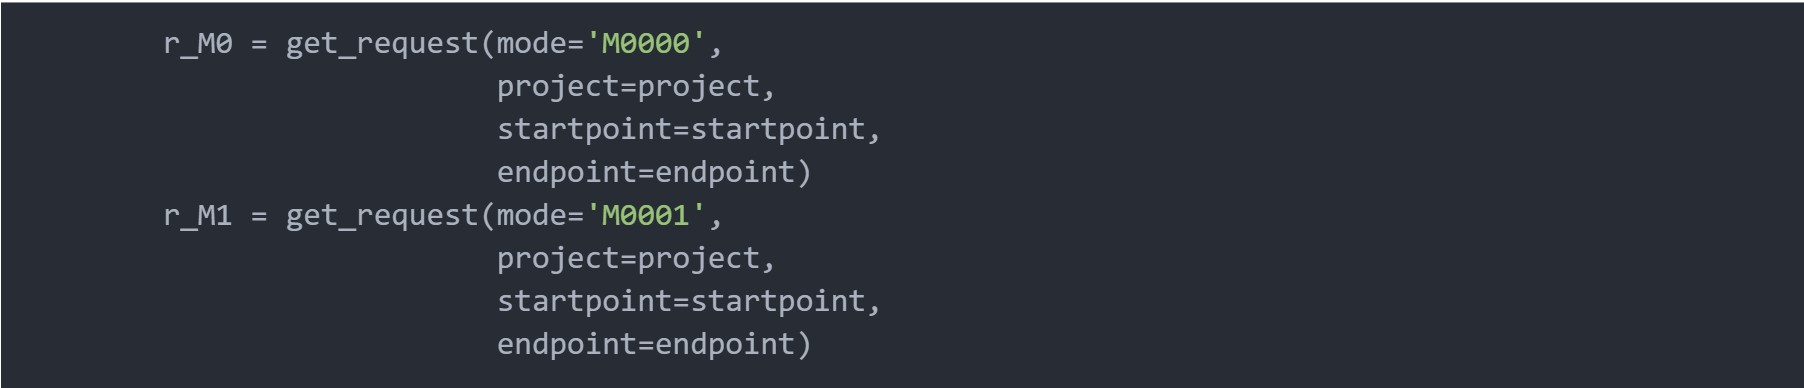
\includegraphics[width=\textwidth]{Figures/3DNavigator/code05.jpg}
    \centering
\end{figure} \vspace{-3.5mm}

Die Funktion “getrequest()” bekommt als Übergabeparameter einen String “mode” übergeben. Dieser Parameter gibt an, um welche Variante der Route es sich handelt. Außerdem wird eine Projekt-ID “project” übergeben. Über diese ID lässt sich das von uns an die API angeforderte Projekt bestimmt. Wir haben diesen Parameter bewusst variabel implementiert, um das gesamte Skript flexibel für einen möglichen weiteren Anwendungsfall im Zusammenhang mit 3D-Navigations APIs von 3d-Berlin zu gestalten. Es werden zudem ein Start “startpoint” sowie ein Endpunkt “endpoint” an die Funktion übergeben. Diese geben an, von welchem Startpunkt aus, welches Ziel zu erreichen sein soll. Es sei dazu gesagt, dass bei jeder Route immer von demselben Startpunkt ausgehen. Dies hat einerseits den Grund, dass der notwendige Datensatz an MP4-Dateien sonst exponentiell steigen würde und wir somit nicht in der Lage während diese Speicherkapazität auf dem Hopper-Server zu gewährleisten. Ebenso setzen wir für unseren Anwendungsfall des Roboters als Hochschulassistenz voraus, dass dieser sich immer an dem gleichen Ort befindet. Es handelt sich bei dem Startpunkt um das Foyer in Haus K. Wir haben auch diesen Parameter dennoch variabel gelassen, um unsere Anwendung so flexibel wie möglich zu entwickeln.

\begin{figure}[H]
    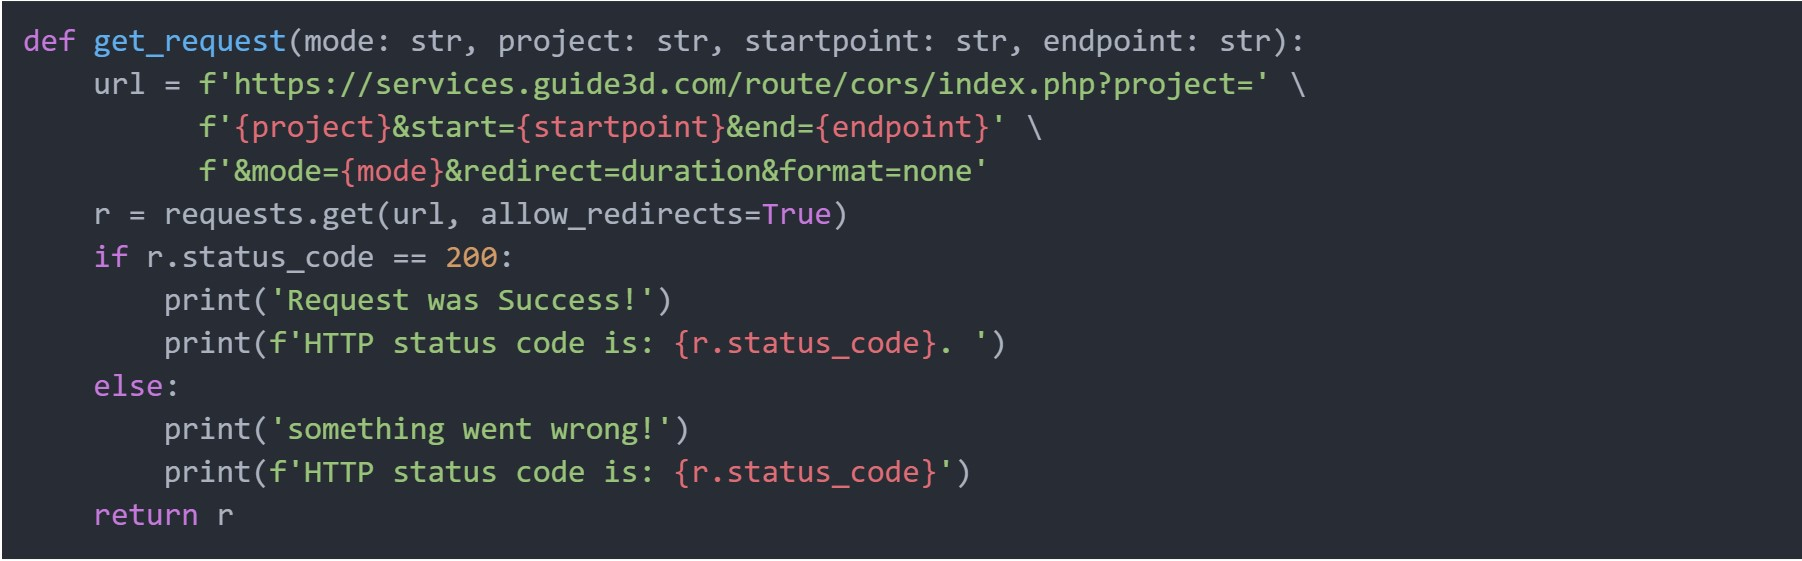
\includegraphics[width=\textwidth]{Figures/3DNavigator/code06.jpg}
    \centering
\end{figure} \vspace{-3.5mm}

Als Nächstes wird über die Liste der Videos iteriert, um den Request für die Anfrage der Routeninformation für genau jedes Video zu erstellen.

\begin{figure}[H]
    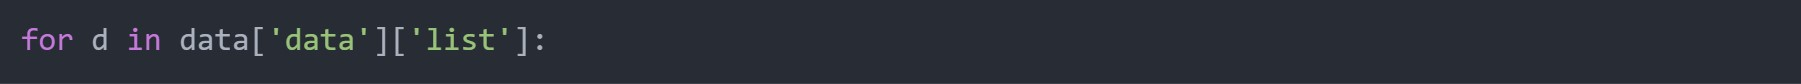
\includegraphics[width=\textwidth]{Figures/3DNavigator/code07.jpg}
    \centering
\end{figure} \vspace{-3.5mm}

Innerhalb dieser Schleife lesen wir als Erstes den Raumnamen und aus der Beschreibung des Ortes ungewollte Zeichen aus dem String heraus. Dies ist notwendig, da es sonst später in der Android-Applikation erfolgen müsste und eine überflüssige Prozessbelastung darstellen würde. Danach werden die Gleitkommazahlen der Dauer und der Distanz einer Route auf ganze Zahlen, als Integer aufgerundet. Außerdem werden die Sekunden in Minuten umgerechnet.

\begin{figure}[H]
    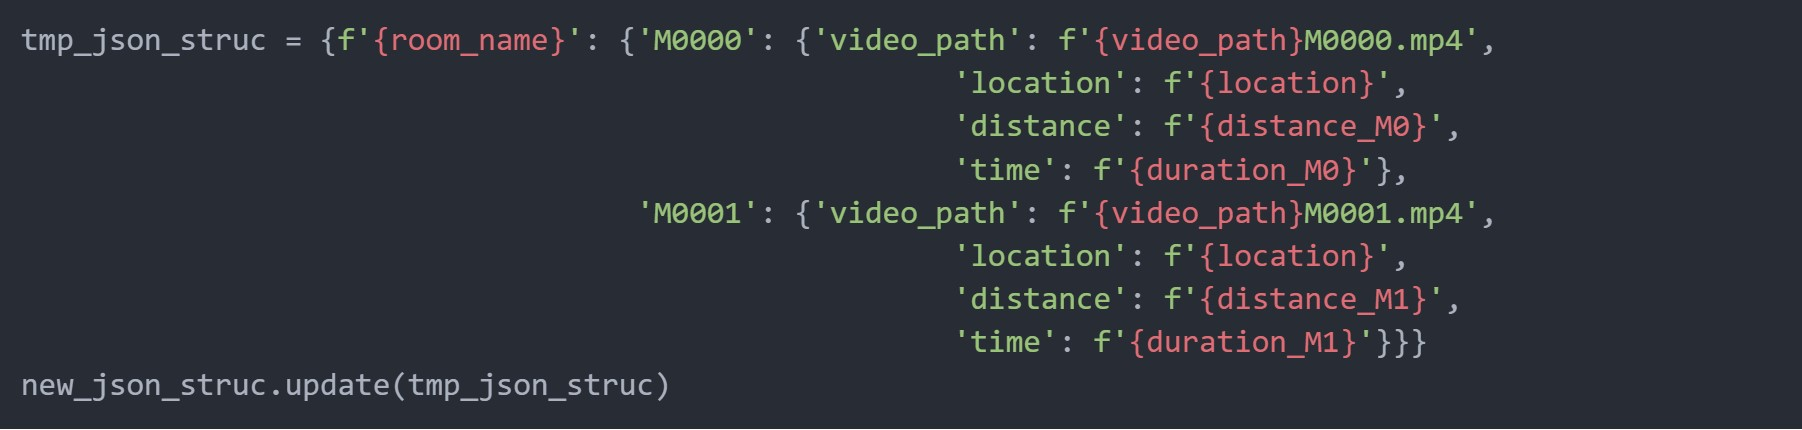
\includegraphics[width=\textwidth]{Figures/3DNavigator/code08.jpg}
    \centering
\end{figure} \vspace{-3.5mm}

Es wird nun ein temporäres JSON-Objekt für die jeweilige Wegroute erzeugt. In dieser wenden wir die zuvor geplante Struktur der Informationen an und weisen die Values den entsprechenden Key zu. Danach wird jedes Objekt an die endgültige JSON-Datei angeknüpft.

\begin{figure}[H]
    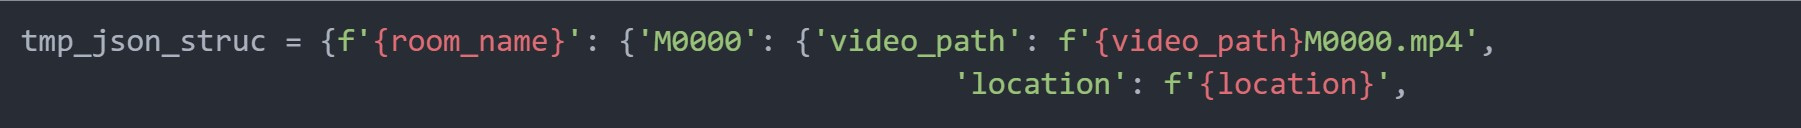
\includegraphics[width=\textwidth]{Figures/3DNavigator/code09.jpg}
    \centering
\end{figure} \vspace{-3.5mm}

Wir haben auch für diese Anwendung nachträglich eine grafische Oberfläche implementiert, um das Ausführen des Programms übersichtlicher und nachhaltiger zu gestalten. Dabei haben wir die Oberfläche so gestaltet, dass wir zwei verschiedene Konsolen für die Outputs anzeigen lassen. Die Linke Ausgabe ist die des Programmablaufs. Auf der rechten Ausgabe sind die hinzugefügten JSON-Objekte aufgelistet. In der folgenden Abbildung ist ein Durchlauf des Programms zu sehen. Es gibt die Möglichkeit ein Zielverzeichnis und den namen für die zu erstellende Datei zu wählen. Werden diese beiden Eigenschaften nicht zuvor gesetzt und mit einem Klick auf die “Submit” Schaltfläche bestätigt, so bekommt die Datei den namen “routedata” und wird in das Verzeichnis “video” geschrieben. Die Abbildung unten zeigt das laufendene Programm:\vspace{-1.5mm}

\begin{figure}[H]
    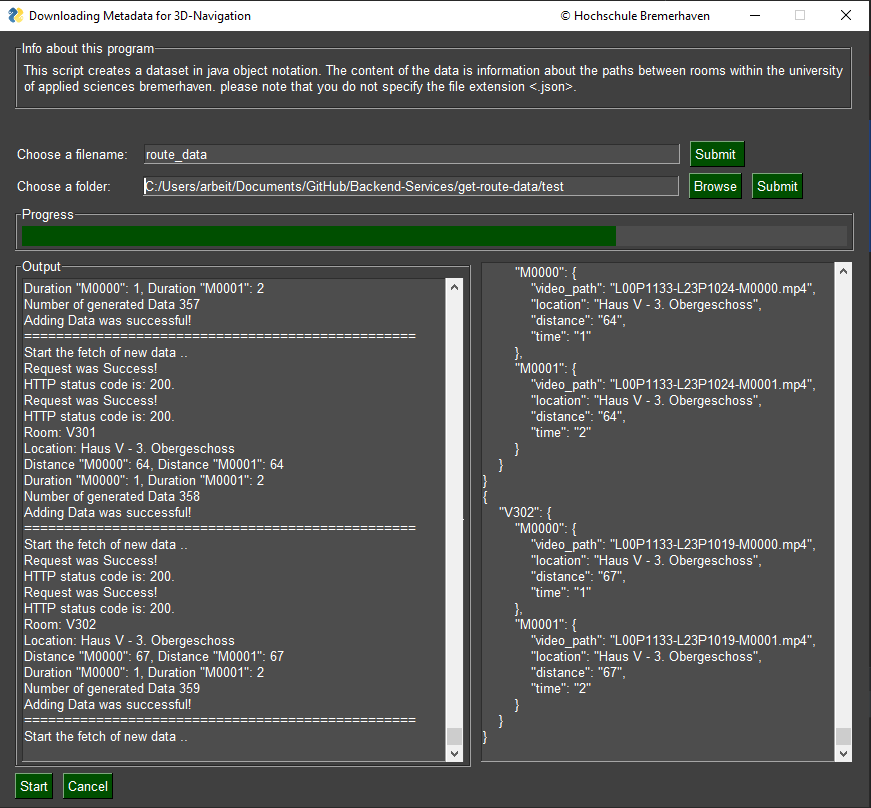
\includegraphics[width=\textwidth]{Figures/3DNavigator/create_metadata_pic_Fertig.png}
    \caption{Screenshot: Grafische Oberfläche des Metadata-Skripts}
    \label{fig:integration}
    \centering
\end{figure}\vspace{-2.5mm}


\section{Sonstiges}
% timetable data
